% Created 2021-09-27 Mon 12:01
% Intended LaTeX compiler: xelatex
\documentclass[letterpaper]{article}
\usepackage{graphicx}
\usepackage{grffile}
\usepackage{longtable}
\usepackage{wrapfig}
\usepackage{rotating}
\usepackage[normalem]{ulem}
\usepackage{amsmath}
\usepackage{textcomp}
\usepackage{amssymb}
\usepackage{capt-of}
\usepackage{hyperref}
\setlength{\parindent}{0pt}
\usepackage[margin=1in]{geometry}
\usepackage{fontspec}
\usepackage{svg}
\usepackage{cancel}
\usepackage{indentfirst}
\setmainfont[ItalicFont = LiberationSans-Italic, BoldFont = LiberationSans-Bold, BoldItalicFont = LiberationSans-BoldItalic]{LiberationSans}
\newfontfamily\NHLight[ItalicFont = LiberationSansNarrow-Italic, BoldFont       = LiberationSansNarrow-Bold, BoldItalicFont = LiberationSansNarrow-BoldItalic]{LiberationSansNarrow}
\newcommand\textrmlf[1]{{\NHLight#1}}
\newcommand\textitlf[1]{{\NHLight\itshape#1}}
\let\textbflf\textrm
\newcommand\textulf[1]{{\NHLight\bfseries#1}}
\newcommand\textuitlf[1]{{\NHLight\bfseries\itshape#1}}
\usepackage{fancyhdr}
\pagestyle{fancy}
\usepackage{titlesec}
\usepackage{titling}
\makeatletter
\lhead{\textbf{\@title}}
\makeatother
\rhead{\textrmlf{Compiled} \today}
\lfoot{\theauthor\ \textbullet \ \textbf{2021-2022}}
\cfoot{}
\rfoot{\textrmlf{Page} \thepage}
\renewcommand{\tableofcontents}{}
\titleformat{\section} {\Large} {\textrmlf{\thesection} {|}} {0.3em} {\textbf}
\titleformat{\subsection} {\large} {\textrmlf{\thesubsection} {|}} {0.2em} {\textbf}
\titleformat{\subsubsection} {\large} {\textrmlf{\thesubsubsection} {|}} {0.1em} {\textbf}
\setlength{\parskip}{0.45em}
\renewcommand\maketitle{}
\author{Houjun Liu}
\date{\today}
\title{Fluid Mosaic Model}
\hypersetup{
 pdfauthor={Houjun Liu},
 pdftitle={Fluid Mosaic Model},
 pdfkeywords={},
 pdfsubject={},
 pdfcreator={Emacs 28.0.50 (Org mode 9.4.4)}, 
 pdflang={English}}
\begin{document}

\tableofcontents



\section{Fluid mosaic model of cell membrane}
\label{sec:orgebae77b}
Some Phosopholipids connected as a "phosolipid bi-layer" (see
\href{KBhBIO101StructuresOfLipids.org}{KBhBIO101StructuresOfLipids}
structure

\begin{itemize}
\item Charged head
\item Nonpolar tail
\end{itemize}

So, head aligns and tail aligns, creating the basic structure of the
membrane:

\begin{figure}[htbp]
\centering
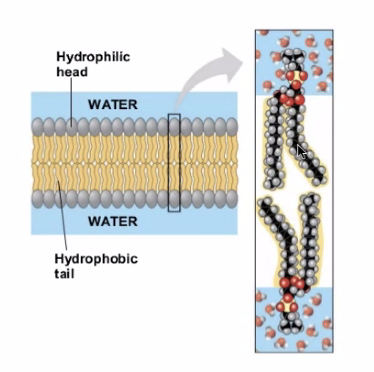
\includegraphics[width=.9\linewidth]{./Screen Shot 2020-09-09 at 3.08.10 PM.png}
\caption{Screen Shot 2020-09-09 at 3.08.10 PM.png}
\end{figure}

This is called the "fluid mosaic" model because there is nothing holding
these together.

\subsection{Stuff in the membrane}
\label{sec:org1867396}
\textbf{Cholesterol}

Helps cells communicate

\textbf{Proteans}

\begin{itemize}
\item Makes sure the right molecules gets in/out
\item Nonpolar Oxygen + CO2 could easily get through
\item Polar and charged molecules can't get through, unless\ldots{}
\item Channeled proteins let specific polar particles through
\end{itemize}

Through various
\href{KBhBIO101CellMembraines.org}{KBhBIO101CellMembraines} protean
transports, chemicals could get in and out of the cell.
\end{document}
